%\documentclass[a4paper]{scrartcl}
%
%% input encoding
%\usepackage[utf8]{inputenc}
%
%% new german spelling
%\usepackage[ngerman]{babel}
%
%% choose font
%\usepackage[T1]{fontenc}
%\usepackage{lmodern}
%\usepackage{dsfont}
%
%% KOMA-Script options
%\KOMAoptions{%
%  parskip=full,%
%  fontsize=12pt,%
%  DIV=calc}
%
%% color and images
%\usepackage{xcolor}
%\usepackage{graphicx}
%\usepackage{wrapfig}
%\usepackage{subcaption}
%\captionsetup{compatibility=false}
%
%% SI units 
%\usepackage{siunitx} 
%
%% quotes
%\usepackage[german=guillemets]{csquotes}
%
%% math
%\usepackage{amsmath}
%\usepackage{amssymb}
%\usepackage{amsfonts} 
%
%% set special behaviour for hyperlinks in pdfs
%\usepackage[breaklinks=true]{hyperref}
%
%% tables don't appear anywhere
%\usepackage{float}
%
%
%% other useful packages 
%\usepackage{enumitem} 
%\usepackage{cancel} 
%\usepackage{wrapfig}
%\usepackage{ booktabs} 
%\usepackage{blindtext}
%
%
%\begin{document}
%\title{V606: Messung der Suszeptibilität paramagnetischer Substanzen}
%\author{Tim Alexewicz (tim.alexewicz@udo.edu), \and Sadiah Azeem (sadiah.azeem@udo.edu)}
%\date{Versuchsdurchführung: 12.04.2022}
%
%\maketitle
%\thispagestyle{empty}
%\newpage
%\thispagestyle{empty}
%\tableofcontents
%\newpage
%\setcounter{page}{1}
%


\section{Auswertung}

\subsection{Filterkurve des Selektivverstärkers}
In \autoref{tab:filterkurve} befinden sich die gemessenen Spannungen $\frac{U_{A}}{U_{E}}$ in Abhängigkeit zur Frequenz $\nu$.
\begin{table}[H]
 \centering 
 \captionabove{Spannungen in Abhängigkeit zur Frequenz}
 \begin{tabular}{cccc} \toprule
 $\nu$ [kHz]& $\frac{U_{A}}{U_{E}}$ [mV] & $\nu$ [kHz]& $\frac{U_{A}}{U_{E}}$ [mV]\\  \midrule
 20.6 & 190 & 33.6 & 2000\\ 
 21.4 & 210 & 34.1 & 2500\\ 
 22   & 220 & 35   & 6900\\
 23.3 & 250 & 36.5 & 4000\\
 24.1 & 280 & 37.2 & 1500\\
 25.6 & 300 & 38.1 & 1200\\
 26.2 & 350 & 39.4 & 900\\
 27   & 430 & 40.2 & 700\\
 28   & 500 & 41.1 & 670\\
 29.4 & 630 & 42   & 600\\
 30.3 & 680 & 43.5 & 490\\
 31.1 & 940 & 44.1 & 430\\
 32.3 & 1100 & 45.2 & 400\\ \bottomrule
 \end{tabular} 
 \label{tab:filterkurve}
\end{table} 
Die Werte aus \autoref{tab:filterkurve} können in eine Gaußfunktion $U(\nu)=a\cdot exp(-(\frac{\nu-b}{c})^2)$ gefittet werden. 
Unter der Benutzung von Matlab ergeben sich für die Parameter $a=7152\ \si{\V}$, $b=35.42$ kHz und $c=1.467$ kHz, 
mit der maximalen Spannung von $U_{max}=7152\ \si{\V}=a$ bei der Frequenz $\nu_{0}=35.42\ \si{\kHz}=b$. 
Die Frequenzen $\nu_{+}$ und $\nu_{-}$ können durch die Beziehung $U(\nu)=\frac{1}{\sqrt{2}}$ berechnet werden. 
Somit ergibt sich für $\nu_{+}=39.875$ und für $\nu_{-}=30.965$. 
Aus $\nu_{0}$, $\nu_{+}$ und $\nu_{-}$ lässt sich die Güte mithilfe von \autoref{eq:guetekuh}
berechnen. Es ergibt sich eine Güte von $Q=3.975$.
\begin{figure}[H]
  \centering
  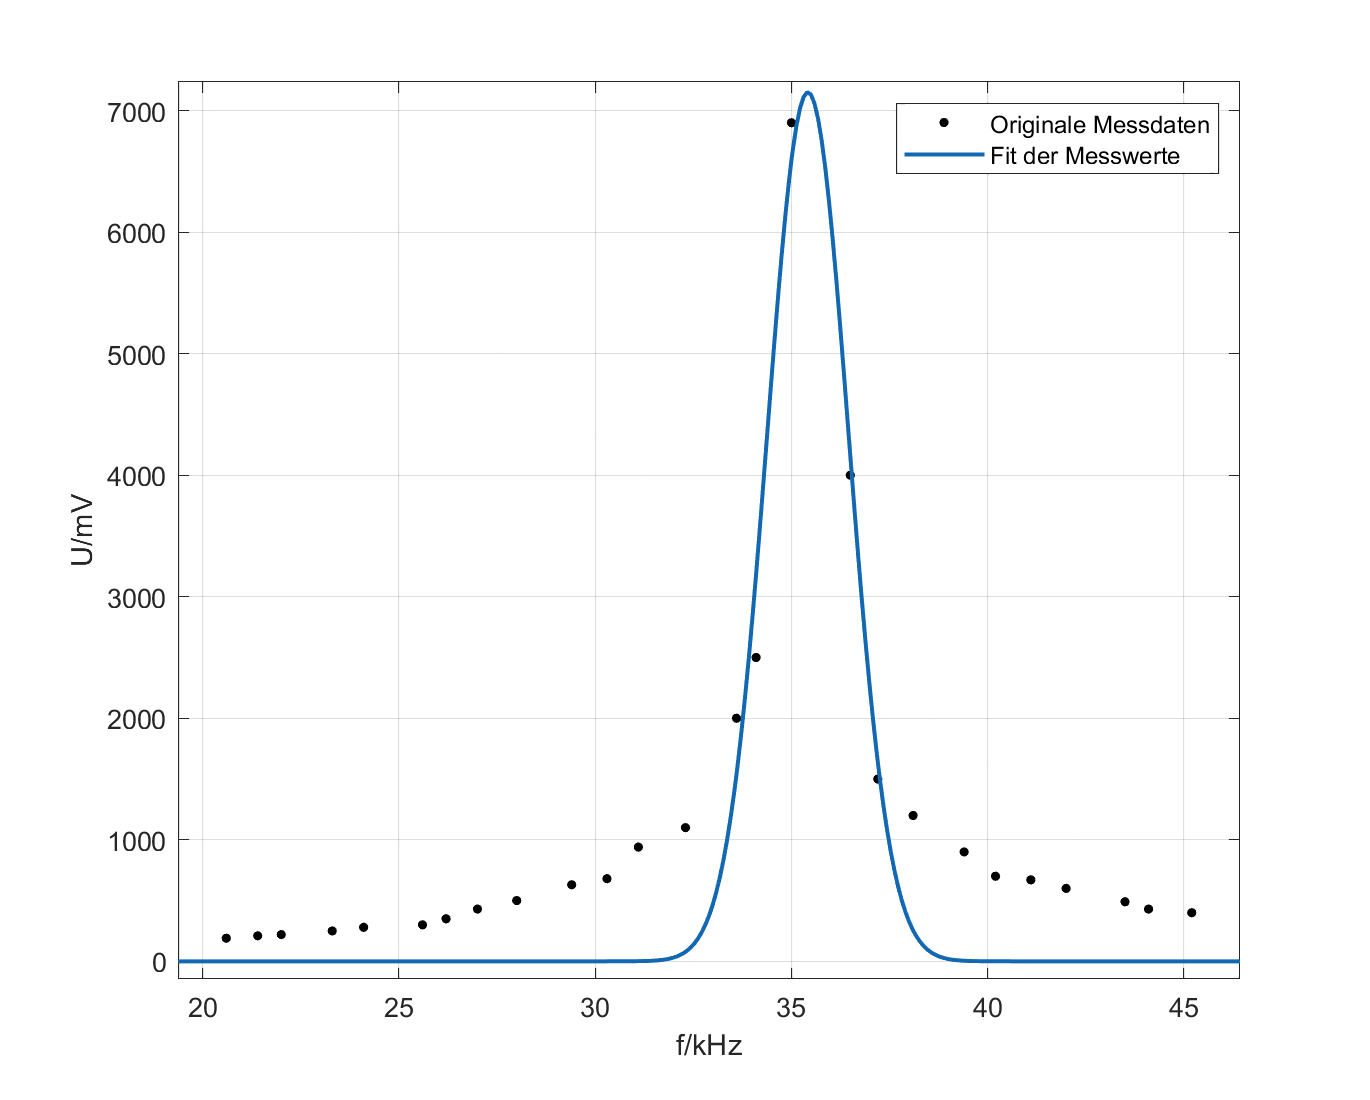
\includegraphics[width=12cm]{content/fit.png}
  \caption{Fit der Messdaten auf eine Gaußfunktion.}
\end{figure}

\subsection{Suszeptibilitäten seltener Erden}
Für den Versuch wurden die Suszeptibilitäten der drei Stoffe $Nd_2 O_3$, $Dy_2 O_3$ und $Gd_2 O_3$ überprüft. Dazu wurde einer Spannung von $1$ V eingespeist. In \autoref{tab:2} befinden sich die niedrigsten Brückenspannungen und Widerstände mit und ohne seltener Erde.
\begin{table}[H]
  \centering
  \caption{Gemessene Spannungen und Widerstände.}
  \begin{tabular}{l|l|l|l|l}
  & $U_{o}$ [mV] & $U_{m}$ [mV] & $R_{o}$ [$\Omega$] & $R_{m}$ [$\Omega$]\\ \hline
  $Nd_2 O_3$ & 300 & 270 & 704 & 667\\
  & 279 & 270 & 708 & 665\\
  & 980 & 990 & 675 & 713\\ \hline
  $Dy_2 O_3$ & 990 & 980 & 670 & 478\\
  & 990 & 980 & 687 & 475\\
  & 990 & 980 & 716 & 472\\ \hline
  $Gd_2 O_3$ & 970 & 970 & 703 & 588\\
  & 970 & 970 & 697 & 590\\
  & 980 & 970 & 675 & 596\\ \hline
  \end{tabular}
  \label{tab:2}
\end{table}\\
Die wichtigsten Größen der Stoffe sind \autoref{tab:3} zu entnehmen,
\begin{table}[H]
  \centering
  \caption{Die wichtigsten Größen der drei Stoffe.}
  \begin{tabular}{l|l|l|l|l|l}
  & m [$\mathrm{g}$] & M [$\mathrm{g/mol}$] & $\rho$ [$\mathrm{g/cm^3}$] & L [$\mathrm{cm}$] & Q [$\mathrm{m^2}$]\\ \hline
  $Nd_2 O_3$ & 18.48 & 336.48 & 7.24 & 15.3 & 1.668$\cdot$10$^{-5}$ \\ \hline
  $Dy_2 O_3$ & 15.10 & 373 & 7.8 & 15.2 & 1.27$\cdot$10$^{-5}$ \\ \hline
  $Gd_2 O_3$ & 14.68 & 363 & 7.4 & 15.3 & 1.30$\cdot$10$^{-5}$ \\ \hline
  \end{tabular}
  \label{tab:3}
\end{table}\\
wobei sich der Querschnitt Q der Probe aus 
\begin{equation*}
  Q=\frac{m}{L\rho}
\end{equation*}
berechnen lässt, m die Masse, M die molare Masse, $\rho$ die Dichte und L die Länge der Probe ist.
Aus den gemessenen Werten ergeben sich die folgenden aufgelisteten mittleren Widerstandsdifferenzen
\begin{align*}
  \bar R_{Nd_2 O_3}&=(0.197 \pm 0.009) \si{\ohm},\\
  \bar R_{Dy_2 O_3}&=(1.083 \pm 0.076) \si{\ohm}\ \textrm{und}\\
  \bar R_{Gd_2 O_3}&=(0.502 \pm 0.055) \si{\ohm}
\end{align*}
aus den Formeln
\begin{align*}
  \bar A&=\frac{1}{n}\sum_{i=1}^n A_i\\
  \Delta A&=\sqrt{\frac{1}{n(n-1)}\sum_{i=1}^n (A_i - \bar A)^2},
  \label{fehler}
\end{align*}
wobei A eine beliebige Größe ist, dessen Mittelwert und Fehler ausgerechnet werden soll und n die Anzahl an Messungen dieser Größe.\\
Aus diesen Mittelwerten ergeben sich mit \autoref{eq:alternativ} und    
\begin{equation}
  \Delta f(A)=\sqrt{\left(\frac{\partial f(A)}{\partial A}\right)^2 (\Delta A)^2}
  \label{gauß}
\end{equation}
die Suszeptibilitäten 
\begin{align*}
  \bar \chi_{Nd_2 O_3}&=(0.00204 \pm 0.00009),\\
  \bar \chi_{Dy_2 O_3}&=(0.0148 \pm 0.0010)\ \textrm{und}\\
  \bar \chi_{Gd_2 O_3}&=(0.0067 \pm 0.0007)
\end{align*}
der seltenen Erden.\\
Über \eqref{eq:1} ergibt sich 
\begin{align*}
  \bar \chi_{Nd_2 O_3}&=(21.04 \pm 13.51),\\
  \bar \chi_{Dy_2 O_3}&=(27.55 \pm 0)\ \textrm{und}\\
  \bar \chi_{Gd_2 O_3}&=(26.74 \pm 0.09)
\end{align*}
für die Suszeptibilitäten. Dabei wurden die drei Spannungen $U_{o}$ und $U_{m}$ aus \autoref{tab:2} pro Stoff mit \eqref{fehler} gemittelt und in \eqref{eq:1} eingesetzt. Dabei ergaben sich die Brücken- und Erregerspannungen
\begin{align*}
  \bar U_{Br_{Nd_2 O_3}}&=(519.67 \pm 230.25) \textrm{mV},\\
  \bar U_{err_{Nd_2 O_3}}&=(513 \pm 238.51) \textrm{mV},\\
  \bar U_{Br_{Dy_2 O_3}}&=(990 \pm 0) \textrm{mV},\\
  \bar U_{Br_{Dy_2 O_3}}&=(980 \pm 0) \textrm{mV},\\
  \bar U_{Br_{Gd_2 O_3}}&=(973 \pm 3.33) \textrm{mV} \textrm{und}\\
  \bar U_{Br_{Gd_2 O_3}}&=(970 \pm 0) \textrm{mV}
\end{align*}
für die Stoffe.\\
Die theoretischen Werte können durch die Hundschen Regeln berechnet werden. Dazu werden der Gesamtdrehimpuls J, der Spin S, der Bahndrehimpuls L und der gyromagnetische Faktor $g_j$ des Moleküls benötigt. Diese sind für die drei Stoffe in \autoref{tab:4} gelistet.
\begin{table}[H]
  \centering
  \caption{Drehimpulse und gyromagnetischer Faktor der einzelnen Stoffe.}
  \begin{tabular}{l|l|l|l|l}
   & J & S & L & $g_j$\\ \hline
   $Nd_2 O_3$ & 9/2 & 3/2 & 6 & 0.72\\ \hline
   $Dy_2 O_3$ & 15/2 & 5/2 & 5 & 1.33\\ \hline
   $Gd_2 O_3$ & 7/2 & 7/2 & 0 & 2\\ \hline
   \end{tabular}
   \label{tab:4}
\end{table}
wobei sich das gyromagnetische Verhältnis aus \autoref{eq:gyromyro} berechnet. 
Wird alles in \autoref{eq:sus} eingesetzt, ergibt sich für die theoretischen Suszeptibilitäten
\begin{align*}
  \chi_{th_{Nd_2 O_3}}&=0.00296\\
  \chi_{th_{Dy_2 O_3}}&=0.02530\\
  \chi_{th_{Gd_2 O_3}}&=0.01377
\end{align*}
wenn für N % aus \eqref{8} --- ist gar nicht in der theorie ---
\begin{equation*}
  N=\frac{Z\rho}{M}\cdot N_{A}
\end{equation*}
genutzt wird, wobei M die molare Masse des Stoffes, $\rho$ die Dichte des Stoffes, $N_A$ die Avogadro-Zahl ist. Für alle Stoffe gilt $Z=2$.

%\section{Diskussion}
%Es wurde mit einer Güte von $Q=20$ gemessen. Die ausgerechnete Güte beträgt allerdings $Q=3.975$. Es lässt sich leicht erkennen, dass das eine große Abweichung ist. 
%Beim Vergleich der Suszeptibilitäten 
%\begin{align*}
%  |\frac{\chi_{th_{N}}-\chi_{exp_{N}}}{\chi_{exp_{N}}}|&=27\ \%\\
%  |\frac{\chi_{th_{D}}-\chi_{exp_{D}}}{\chi_{exp_{D}}}|&=15\ \%\\
%  |\frac{\chi_{th_{G}}-\chi_{exp_{G}}}{\chi_{exp_{G}}}|&=3\ \%
%\end{align*}
%wird bemerkbar, dass die ersten beiden Stoffe zu extrem abweichen und die Auswertung keine reliable Zustimmung der Theorie ist und dementsprechend beim Messvorgang etwas falsch abgelesen wurde, zum Beispiel die 10 mV Skala mit der 30 mV Skala verwechselt wurde, oder die Rundungen für die starken Abweichungen gesorgt haben. Beim dritten Molekül ergibt sich alles wunderbar und die Abweichung ist noch im Signifikanzintervall, bestätigt also als Einziges die Theorie. 

%\section{Literaturverzeichnis}
%
%[1] Technische Universität Dortmund, \textit{V606: Messung der Suszeptibilität paramagnetischer
%Substanzen}
%
%
%
%\end{document}
%
